\section*{Zusammenfassung}

Der Übergang von einem Bild in ein Anderes kann durch verschiedene
Effekte erreicht werden. Einer der bekanntesten ist die sogenannte
Kreuzblende (engl. cross dissolve). Dabei wird jeder Pixel des Quellbildes
sukzessive um (1-1/numIterations) abgeschwächt und dafür jeder Pixel
des Zielbildes um 1/numIterations multipliziert (verstärkt). 
Das Resultat aus der Addition dieser beiden Operationen ergibt den
Effekt der eben genannten Kreuzblende:

\begin{equation}	
	\left( 1-\frac{1}{numIterations} \right) \cdot \mathbf{x} + \frac{1}{numIterations} \cdot \overline{\mathbf{x}}
\end{equation}




\begin{figure}
	
	\centering
	\begin{subfigure}{0.4\textwidth}
		\centering
		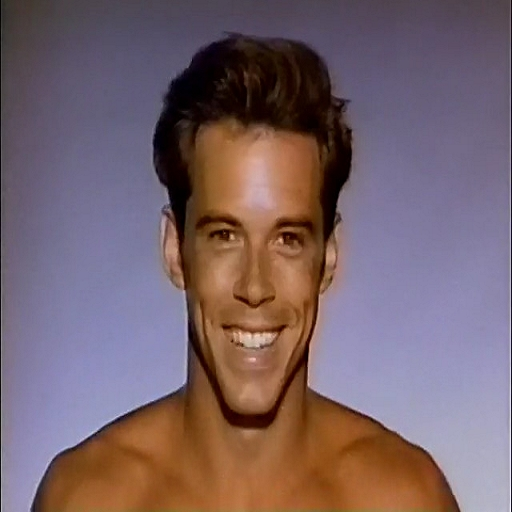
\includegraphics[width=\linewidth]{guy_squared.jpg}
		\caption{Quellbild}
		\label{fig:source}
	\end{subfigure}
	\hfill
	\begin{subfigure}{0.4\textwidth}
		\centering
		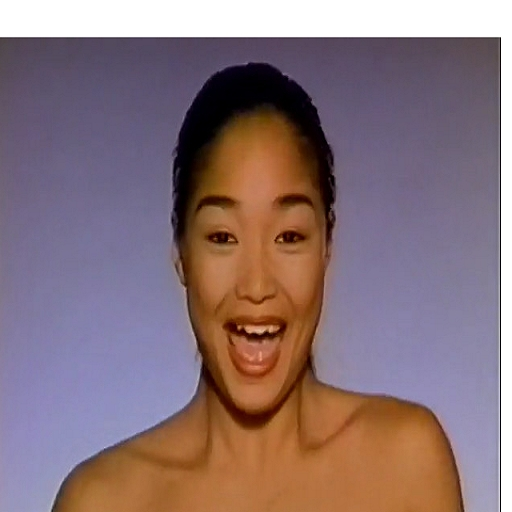
\includegraphics[width=\linewidth]{gal_squared.jpg}
		\caption{Zielbild}
		\label{fig:dest}
	\end{subfigure}
	
	\centering
	\begin{subfigure}{0.4\textwidth}
		\centering
		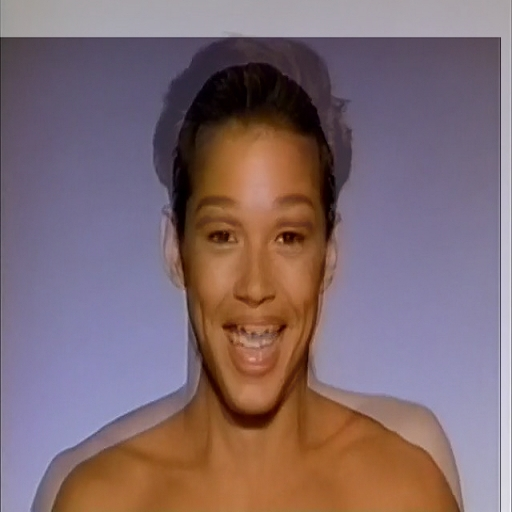
\includegraphics[width=\linewidth]{cross_dissolve_50pct.jpg}
		\caption{50\% Kreuzblende}
		\label{fig:dissolve}
	\end{subfigure}
	\hfill
	\begin{subfigure}{0.4\textwidth}
		\centering
		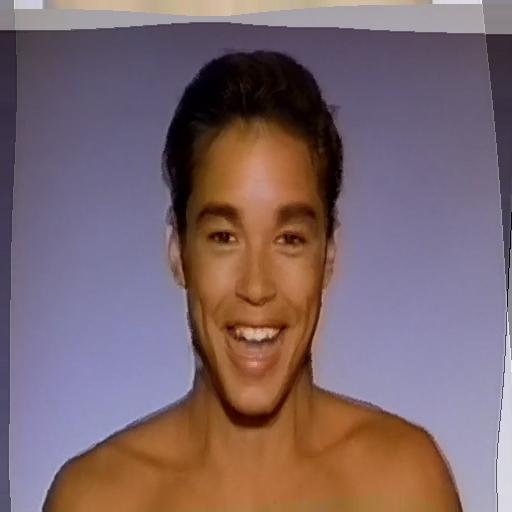
\includegraphics[width=\linewidth]{beierneely_50_pct.jpg}
		\caption{50\% Beier-Neely Morph}
		\label{fig:morph}
	\end{subfigure}
	\caption{}
	\label{fig:side-by-side}
	
\end{figure}
